\documentclass[11pt]{article}
\usepackage[margin=2.6cm]{geometry}
\usepackage{amsmath,amssymb}
\usepackage{graphicx}
\usepackage[colorlinks=true,linkcolor=blue,citecolor=blue,urlcolor=blue]{hyperref}
\usepackage{booktabs}
% AUTO-GENERATED by scripts/make_paper_numbers.py — DO NOT EDIT
% source commit: 3d8fdbb
\newcommand{\NmAndEta}{11.53}
\newcommand{\NmAndMf}{9.5\times10^{-16}}
\newcommand{\NmAndMfArr}{9.1\times10^{-31}}
\newcommand{\NmSgrEta}{6.947}
\newcommand{\NmSgrMf}{8.9\times10^{-10}}
\newcommand{\NmSgrMfArr}{7.9\times10^{-19}}
\newcommand{\NmTraEta}{0.740}
\newcommand{\NmTraMf}{0.108}
\newcommand{\NmProxEta}{0.0849}
\newcommand{\NmProxMf}{0.775}
\newcommand{\NmProxEtaRT}{0.169}
\newcommand{\NmTraEtaRT}{1.260}
\newcommand{\NmSgrEtaRT}{7.640}
\newcommand{\NmAndEtaRT}{12.22}
\newcommand{\NmTflQ}{2.58\times10^{3}}
\newcommand{\NmTeffQ}{1.22}
\newcommand{\NmTceilQ}{0.824}
\newcommand{\NmTflXII}{5.98\times10^{18}}
\newcommand{\NmTeffXII}{31.1}
\newcommand{\NmTceilXII}{30.4}
\newcommand{\NmXstar}{0.54}
\newcommand{\NmLamstar}{0.13}
\newcommand{\NmEtaFb}{0.366}
\newcommand{\NmMassMsunKm}{0.102}
\newcommand{\NmMassKgKm}{2.02\times10^{29}}
\newcommand{\NmLpeakW}{3.1\times10^{51}}
\newcommand{\NmLpeakLsun}{8.1\times10^{24}}
\newcommand{\NmBurnMuS}{17.6}
\newcommand{\NmRadEtaQ}{51.3}
\newcommand{\NmSeatXII}{2.6\times10^{10}}
\newcommand{\NmGRowsP}{306}
\newcommand{\NmSigRows}{567}
\newcommand{\NmMapMission}{5.0\times10^{-15}}
\newcommand{\NmMapRide}{1.06\times10^{-6}}
\newcommand{\NmFlashPeak}{1.48\times10^{4}}
\newcommand{\NmFlashExp}{72}
\newcommand{\NmFlashDecay}{5\times10^{-6}}
\newcommand{\NmFlashPs}{15}
\newcommand{\NmWtCommit}{1e9e3db}
\newcommand{\NmRepoCommit}{3d8fdbb}


\title{Interstellar flight profiles and observational signatures of\\
positive-energy warp shells}
\author{[Author Name]\\ \small Independent Researcher, Tokyo\\
\small ORCID: [to be supplied]}
\date{2026}

\begin{document}
\maketitle

\begin{abstract}
Accelerating warp shells built entirely from positive-energy matter were
recently shown to exist: the radiative momentum warpshell of
Le~\cite{le-steering} steers by photon-rocket recoil under a closed-form
cost law and an acceleration--compactness frontier. What that construction
does not contain is a flight plan. A systematic search (a citation scan, a
full-text survey of the paper, and an inspection of the author's public
reproduction code) found no published computation of interstellar routes
under the shell's admissibility constraints. We compute that catalog. Under
the full constraint stack, a rigorous ceiling, a numerically mapped
frontier band, and a provisional rigorous floor, we obtain fuel--time
tables for Proxima Centauri, TRAPPIST-1, Sgr~A*, and M31; the crew-lifetime
contour ($\tau = 50$~yr) requires cruise rapidity $\eta = \NmAndEta$ for an
M31 flyby at mass ratio $m_f/m_0 = \NmAndMf$. Time-optimal profiles ride
the moving frontier, and the operative constraint switches from the
thin-shell frontier to thick-wall realizability at compactness
$x^* \approx \NmXstar$. The same integrals yield observational signatures:
a saturated accelerating shell is exactly dark toward its destination, and
announces arrival with a deceleration flash amplified by $\delta^4 =
e^{4\eta}$ and compressed in arrival time, following the general decay law
$F \propto e^{7\eta - 3\Delta\eta_{\rm tot}}$ (for the M31 arrival,
$e^{7\eta-\NmFlashExp}$, with picosecond-scale structure), while remaining
gravitationally silent on the Damour dipole. All numbers are
machine-injected from certified catalogs ($\NmGRowsP$ catalog rows and
$\NmSigRows$ signature rows, dual-path verified with zero omissions); the
verification record includes six cross-validations against the author's
code and one reproducibility gap, which we state as found.
\end{abstract}

\section{Introduction}\label{sec:intro}

The warp-drive literature has split into two lines that have not met. One
line proves what a shell can be. Alcubierre's metric~\cite{alcubierre}
required negative energy, and the no-go results of Santiago, Schuster, and
Visser~\cite{ssv}, together with the quantum-inequality bounds of Pfenning
and Ford~\cite{pfenning} and the eigenvalue analysis of Lobo and
Visser~\cite{lobo}, established that the defect is generic for
metric-first designs. The positive-energy soliton of Lentz~\cite{lentz}
did not survive scrutiny: the Eulerian energy density of the zero-vorticity
soliton integrates to zero over each slice~\cite{ssv}, and a direct
Eulerian-frame computation exhibits the negative regions~\cite{celmaster}.
Source-first constructions then produced genuinely positive-energy shells,
static or at constant velocity: the taxonomy of Bobrick and
Martire~\cite{bobrick} and the numerically verified constant-velocity
shells of Fuchs \emph{et al.}~\cite{fuchs}, built with the Warp Factory
toolkit~\cite{helmerich}. Le closed the acceleration gap: the radiative
momentum warpshell~\cite{le-steering} wraps a flat passenger cavity in a
timelike shell matched to the exact Kinnersley photon
rocket~\cite{kinnersley}, satisfies the dominant energy condition in bulk
and on the shell, and steers under the closed-form control law $-\dot m
\geq 3m|a|$ with a Tsiolkovsky budget $m_f/m_0 = e^{-3\Delta\eta}$.

The other line computes where a point mass can fly.
F\"uzfa~\cite{fuzfa2019} modeled interstellar travel aboard the bare
Kinnersley rocket, deriving trajectories, energy costs, aberration, and
Doppler shifts for Proxima-bound missions, and extended the astronautics
to laser-pushed sails in a companion study~\cite{fuzfa2020}. Those
computations carry no passenger cavity, no matched shell, and none of the
admissibility constraints that make the shell physical.

A systematic search --- a citation scan of arXiv:2606.22531 (Semantic
Scholar and INSPIRE-HEP, 2026-08-08, zero citing records), a full-text
survey of v3, and an inspection of the author's public reproduction code
at commit \NmWtCommit{}~\cite{worldtube} --- found no published computation
of interstellar flight profiles under the shell's admissibility
constraints. The present paper performs that computation and derives its
observable consequences.

This paper contributes four items. First, an admissibility-constrained
maneuver catalog: a destination-free rapidity ladder, mission tables for
four destinations with the crew-lifetime contour, and the seat price of
carrying passengers relative to an ideal photon rocket. Second,
time-optimal profiles in a three-tier constraint system, including a
constraint-regime crossover at $x^* \approx \NmXstar$ (to our knowledge
not previously quantified; Sec.~\ref{sec:results}C). Third, a signature
catalog mapping every
profile to observer-frame light curves, with an exact forward null during
saturated acceleration, a deceleration flash governed by a general
closed-form decay law, and a gravitational-wave silence discriminator.
Fourth, a verification methodology (certification tests, dual-path checks,
authority labels, and human decision gates over an AI workflow) whose
record includes six cross-validations against the author's code and one
reproducibility gap, reported factually in Sec.~\ref{sec:methods}.

\section{Framework}\label{sec:framework}

We use the framework of Ref.~\cite{le-steering} as published and do not
re-derive it. The exterior is the Kinnersley--Robinson--Trautman photon
rocket sourced by outgoing null dust; its rest-frame exhaust pattern is
the exact dipole $4\pi n^2(\vartheta) = -\dot m - 3ma\cos\vartheta$
(Eq.~(13) of Ref.~\cite{le-steering}), with $\vartheta$ measured from the
proper-acceleration axis in the momentary rest frame. Bulk energy
conditions reduce to $n^2 \geq 0$, whose forward-pole binding yields the
control law $-\dot m \geq 3m|a|$ (Eq.~(14)) and the budget $m_f/m_0 =
e^{-3\int|a|\,du}$ (Eq.~(15)). The static anchor satisfies the surface
dominant energy condition for $x = 2m/R < 24/25$ (Eq.~(25)); a regular
exterior foliation caps the acceleration at the kinematic ceiling
$\lambda = aR < \tfrac{1}{2}(1-x)$ (Eq.~(40)); and finite-thickness
(tangential-pressure) realizability requires the rear-pole effective
compactness to satisfy $x + 2\lambda < 4/5$ (Sec.~10 of
Ref.~\cite{le-steering}).

Every number we publish inherits an authority label from the source
theory, following the paper's own distinction between rigorous closed
forms, numerical maps, and heuristics. Label [R] marks exact closed forms;
[N] marks reliance on published numerics, used strictly inside the sampled
domain; [H] marks heuristics, displayed but never used as constraints. The
operative constraint system is three-tiered (Table~\ref{tab:tiers}): a
rigorous ceiling $\min\{\tfrac12(1-x), \tfrac12(\tfrac45 - x)\}$ [R]; the
effective band $\underline{g}(x)$ [N], the observer-robust frontier scan
of Ref.~\cite{le-steering} on $x \in [0.1, 0.7]$; and a floor $c_{\rm
cons}(x)$, a conservative independent evaluation of the paper's rigorous
lower-bound chain, carried provisionally for the reason recorded in
Sec.~\ref{sec:methods}. All riding profiles additionally impose the
ceiling as a hard clamp.

\begin{table}[t]
\centering
\caption{The three-tier constraint system on $\lambda = aR$.}
\label{tab:tiers}
% AUTO-GENERATED by scripts/make_paper_numbers.py — DO NOT EDIT
\begin{tabular}{llll}
\hline
Tier & Bound on $\lambda=aR$ & Authority & Domain \\
\hline
Ceiling & $\min\{\tfrac12(1-x),\,\tfrac12(\tfrac45-x)\}$ & [R] (unattainable upper limit) & $x\in(0,4/5)$ \\
Effective & $\underline{g}(x)$, linear interpolation & [N] (no extrapolation) & $x\in[0.1,0.7]$ \\
Floor & $c_{\rm cons}(x)$ & [R(A3)/provisional] & $x\in(0,4/5)$ \\
\hline
\end{tabular}

\end{table}

\section{Methods}\label{sec:methods}

\subsection{Verification protocol}

The computation is organized as a verified pipeline rather than a single
code. Equations enter through a formula ledger transcribed from the source
paper (v3 throughout; the v2 to v3 equation renumbering is mapped in the
ledger); every implemented equation carries a certification test that
reproduces a value printed in the paper before it may be used downstream.
The certification suite contains eighteen gates (C1--C18), from the
Tsiolkovsky budget and the surface energy-condition window through the
observer-frame pattern normalization of the signature layer. Principal
quantities are computed along two independent paths (closed form against
independent numerics), and disagreement is a stop condition rather than a
tolerance to be widened silently: the catalog carries \NmGRowsP{} verified
rows in the maneuver layer and \NmSigRows{} rows in the signature layer,
with zero omissions.

Two path-agreement tolerances apply. Closed-form-capable rows meet
$10^{-8}$, and the mission-class retarded-time maps agree to
$\NmMapMission$. For frontier-riding profiles the two implementations of
the retarded-time map agree to $\NmMapRide$ against a documented class
tolerance of $2\times10^{-6}$: the stored ride grids information-limit the
interpolation (kinks of the piecewise-linear $\underline{g}$ fall inside
grid intervals, and the early-burn $\lambda$ gradient at $x_0=0.7$ is
steep), so the residual reflects the consumed data, not the
implementations. This class tolerance was itself ratified at a human
decision gate (2026-08-09) under a project rule that tolerance changes are
human-approval items.

All numerical claims in this paper, including table entries and figure
captions, are machine-injected from the certified catalogs through a
generated macro layer; a manifest records the source field and display
transform of every injected value, and a certification test scans the
manuscript for bare numeric literals and recomputes the manifest.

\subsection{AI involvement}

All computations, implementations, and manuscript drafting were performed
by Claude (Fable 5, Anthropic) under a human-gated protocol: every phase
deliverable was reviewed and approved at explicit human decision gates,
all numerical claims are machine-injected from the certified catalogs, and
tolerance changes were themselves human-gate items.

\subsection{Cross-validation against the author's code and one gap}

We pinned the author's public reproduction code~\cite{worldtube} at commit
\NmWtCommit{} and obtained six agreements: the frontier pins
$\underline{g}(x)$ match our transcription verbatim; the axial margin
formula (Eq.~(42) of Ref.~\cite{le-steering}) matches token for token; the
quoted worst ratio of the frozen axial threshold to the ceiling
($0.9931$ at $x \approx 0.631$) is reproduced independently from our own
transcriptions; the stated accuracy domain of the closed-form estimate is
confirmed on its stated range; the frozen-margin coefficients agree
symbolically; and the code states explicitly that the v2 bifurcation
scalar was removed in v3, confirming a structural retraction we had
identified independently and quarantined in our harness.

One quantity resisted verification. The evaluated floor values of Eq.~(73)
could not be independently reproduced from the paper text and the public
code; the three suprema they require are described procedurally in both
sources but given in closed form in neither. We therefore constructed a
conservative independent floor and label it provisionally. Our
$c_{\rm cons}(x)$ evaluates strictly below the printed values at all five
sampled compactnesses and reproduces the printed binding-branch structure;
because every step of its chain is either a printed closed form or a
provable over-estimate under a documented reading, it is a true lower
bound within that reading. The discrepancy is recorded as a
reproducibility statement, not as an error claim, and the floor tier of
every product in this paper carries the provisional label.

\section{Results}\label{sec:results}

\subsection{The rapidity ladder and the seat price}

Fuel is destination-free: $m_f/m_0 = e^{-3\Delta\eta}$ depends only on the
integrated rapidity, so the first catalog table (Table~\ref{tab:ladder})
has no distance column. The mandatory dipole breadth of the news-silent
exhaust makes the passenger shell pay $e^{3\eta}$ where an ideal
collimated photon rocket pays $e^{\eta}$; the seat price, their ratio, is
$e^{2\eta}$. At the worked-burn rapidity $\eta = 0.24$ the shell radiates
$\NmRadEtaQ\%$ of its rest mass (matching the source paper's worked
maneuver, which our suite reproduces as certification C4), and the seat
price is a modest $1.6$; at $\eta = 12$ the seat price reaches
$\NmSeatXII$.

\begin{table}[t]
\centering
\caption{Rapidity ladder (destination-free, all [R]). The $1-\beta$
column resolves the approach to light speed where $\beta$ saturates the
displayed digits; the seat price is the initial-mass ratio relative to an
ideal collimated photon rocket.}
\label{tab:ladder}
% AUTO-GENERATED by scripts/make_paper_numbers.py — DO NOT EDIT
\begin{tabular}{rrrrrr}
\hline
$\eta$ & $\beta$ & $1-\beta$ & $m_f/m_0$ & radiated & seat price $e^{2\eta}$ \\
\hline
0.24 & 0.2355 & $7.6\times10^{-1}$ & $4.9\times10^{-1}$ & 51.3\% & $1.6\times10^{0}$ \\
1 & 0.7616 & $2.4\times10^{-1}$ & $5.0\times10^{-2}$ & 95.0\% & $7.4\times10^{0}$ \\
3 & 0.9951 & $4.9\times10^{-3}$ & $1.2\times10^{-4}$ & 100.0\% & $4.0\times10^{2}$ \\
5 & 0.9999 & $9.1\times10^{-5}$ & $3.1\times10^{-7}$ & 100.0\% & $2.2\times10^{4}$ \\
8 & 1.0000 & $2.3\times10^{-7}$ & $3.8\times10^{-11}$ & 100.0\% & $8.9\times10^{6}$ \\
12 & 1.0000 & $7.6\times10^{-11}$ & $2.3\times10^{-16}$ & 100.0\% & $2.6\times10^{10}$ \\
\hline
\end{tabular}

\end{table}

\subsection{Mission tables and the crew-lifetime contour}

Mission kinematics (hyperbolic burns, coast at fixed rapidity) convert the
ladder into timetables for four destinations (Proxima Centauri,
TRAPPIST-1, Sgr~A*, M31; catalog distances fixed with sources in the data
release). Burn durations are microseconds for kilometer-scale shells, so
mission times are cruise-dominated, and the ship proper time is
$\tau \approx D/\sinh\eta$. Table~\ref{tab:contour} reports the
crew-lifetime contour $\tau = 50$~yr: a Proxima flyby needs only
$\eta = \NmProxEta$ at mass ratio $\NmProxMf$; Sgr~A* needs
$\eta = \NmSgrEta$ at $\NmSgrMf$; an M31 flyby needs $\eta = \NmAndEta$ at
$m_f/m_0 = \NmAndMf$. Arrival (deceleration into the destination system)
doubles the exponent, and a round trip quadruples it: the M31 arrival
costs $\NmAndMfArr$, which prices the mission rather than forbidding it,
since the budget is positive-energy throughout. For round trips the
lifetime condition applies to the total out-and-back proper time, so the
round-trip column of Table~\ref{tab:contour} is evaluated at its own
cruise rapidity $\eta_{\rm RT} = {\rm arcsinh}(2D/\tau)$ (for M31,
$\eta_{\rm RT} = \NmAndEtaRT$), and its fuel column uses $\Delta\eta_{\rm
tot} = 4\eta_{\rm RT}$. Figure~\ref{fig:contour} shows the contour across
the ladder.

\begin{table}[t]
\centering
\caption{Crew-lifetime contour ($\tau = 50$~yr, ship proper time; burns
included exactly, cruise-dominated). The flyby and arrival columns share
$\eta_{50} = {\rm arcsinh}(D/\tau)$; the round-trip column is evaluated at
its own $\eta_{\rm RT} = {\rm arcsinh}(2D/\tau)$, the rapidity at which
the total out-and-back proper time meets the contour. Fuel columns are
$m_f/m_0 = e^{-3\Delta\eta_{\rm tot}}$ with $\Delta\eta_{\rm tot} =
\eta_{50}, 2\eta_{50}, 4\eta_{\rm RT}$.}
\label{tab:contour}
% AUTO-GENERATED by scripts/make_paper_numbers.py — DO NOT EDIT
\begin{tabular}{lrrrrrr}
\hline
Destination & $D$ [ly] & $\eta_{50}$ & $\eta_{\rm RT}$ & $m_f/m_0$ (flyby) & (arrive) & (round trip) \\
\hline
Proxima Centauri & 4.25 & 0.085 & 0.169 & 7.8e-01 & 6.0e-01 & 1.3e-01 \\
TRAPPIST-1 & 40.5 & 0.740 & 1.260 & 1.1e-01 & 1.2e-02 & 2.7e-07 \\
Sgr A* & $2.6\times10^{4}$ & 6.947 & 7.640 & 8.9e-10 & 7.9e-19 & 1.5e-40 \\
M31 (Andromeda) & $2.54\times10^{6}$ & 11.529 & 12.222 & 9.5e-16 & 9.1e-31 & 2.0e-64 \\
\hline
\end{tabular}

\end{table}

\begin{figure}[t]
\centering
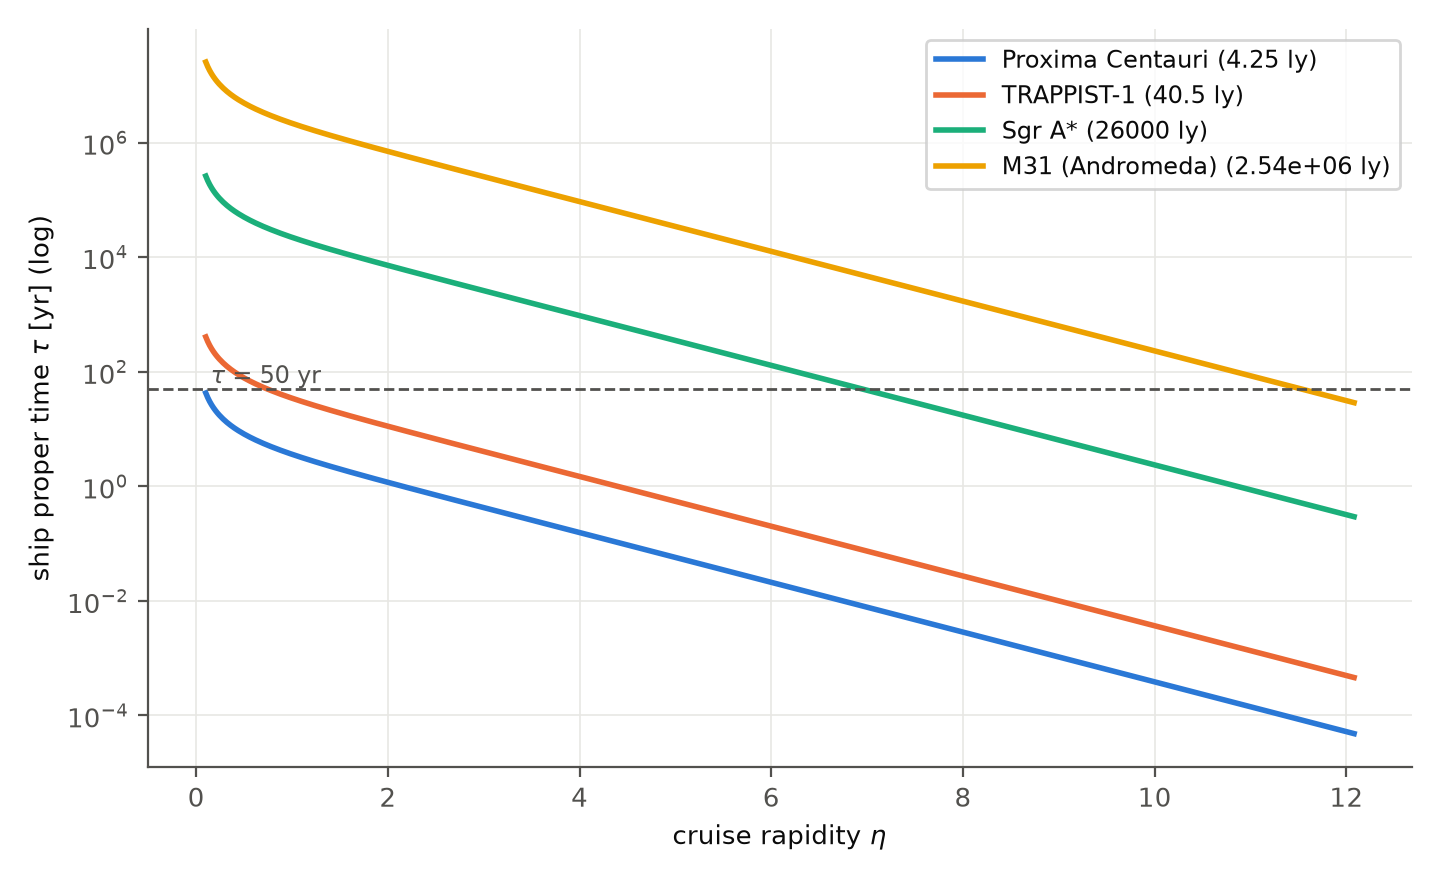
\includegraphics[width=0.82\linewidth]{figures/fig1_contour.png}
\caption{Ship proper time versus cruise rapidity for arrival missions to
the four catalog destinations, with the 50-year contour marked. Crossings
occur at the $\eta_{50}$ values of Table~\ref{tab:contour}.}
\label{fig:contour}
\end{figure}

\subsection{Three-tier time-optimal profiles and the constraint-regime
crossover}

The time-optimal maneuver at fixed $\Delta\eta$ saturates the frontier
almost everywhere (Theorem~8 of Ref.~\cite{le-steering}), so the minimum
time is the quadrature $T = R\int_0^{\Delta\eta} d\eta'/
\lambda_{\rm tier}(x_0 e^{-3\eta'})$ along the moving wall: the shell
radiates, $x$ falls, and the wall widens during the burn. We evaluate this
riding time in all three tiers (Fig.~\ref{fig:bracket},
Table~\ref{tab:bracket}). The effective [N] band leaves its sampled domain
at $\eta_{\rm fb} = \ln(x_0/0.1)/3 = \NmEtaFb$ (for $x_0 = 0.3$) and falls
back to the rigorous ceiling, with the fallback point recorded in every
profile; for $\Delta\eta \gtrsim 1$ the effective and ceiling times
converge, so the bracket tightens automatically. The floor tier is slower
by orders of magnitude and grows as $e^{3\Delta\eta}$; this is the
conservatism of a proof, not a property of nature, and in SI units even
the floor-tier burn at $\Delta\eta = 0.24$ lasts milliseconds for
$R = 1$~km.

The three tiers also locate a structural fact about the constraint stack
(Fig.~\ref{fig:tiers}). The thin-shell frontier scan $\underline{g}(x)$
[N] crosses the thick-wall ceiling $(4/5 - x)/2$ [R] at $x^* \approx
\NmXstar$ ($\lambda^* \approx \NmLamstar$, under the linear interpolation
of the published pins): below $x^*$ the dominant-energy frontier binds,
above it thick-wall realizability binds, and thin-shell catalog values
beyond $x^*$ are reachable only in the distributional idealization. To our
knowledge, within the scope of the systematic search described in
Sec.~\ref{sec:intro}, this crossover has not been quantified before. The
physical content is consistent with the source paper's own nesting of
admissibility windows; the crossover simply makes the switch of operative
regime quantitative.

\begin{table}[t]
\centering
\caption{Frontier-riding minimum times at $x_0 = 0.3$ (units of $R$;
multiply by $R/c$ for SI). The ceiling column is an unattainable lower
bound (the ceiling is an open condition); the fallback column marks where
the [N] band exits its sampled domain.}
\label{tab:bracket}
% AUTO-GENERATED by scripts/make_paper_numbers.py — DO NOT EDIT
\begin{tabular}{rrrrr}
\hline
$\Delta\eta$ & $T_{\rm floor}/R$ & $T_{\rm eff}/R$ & $T_{\rm ceil}/R$ & $\eta_{\rm fb}$ \\
\hline
0.1 & 1e+03 & 0.515 & 0.37 & -- \\
0.24 & 2.58e+03 & 1.22 & 0.824 & -- \\
0.5 & 6.88e+03 & 2.25 & 1.57 & 0.366 \\
1 & 3.01e+04 & 3.56 & 2.88 & 0.366 \\
2 & 5.65e+05 & 6.08 & 5.39 & 0.366 \\
3 & 1.12e+07 & 8.58 & 7.89 & 0.366 \\
5 & 4.53e+09 & 13.6 & 12.9 & 0.366 \\
8 & 3.67e+13 & 21.1 & 20.4 & 0.366 \\
12 & 5.98e+18 & 31.1 & 30.4 & 0.366 \\
\hline
\end{tabular}

\end{table}

\begin{figure}[t]
\centering
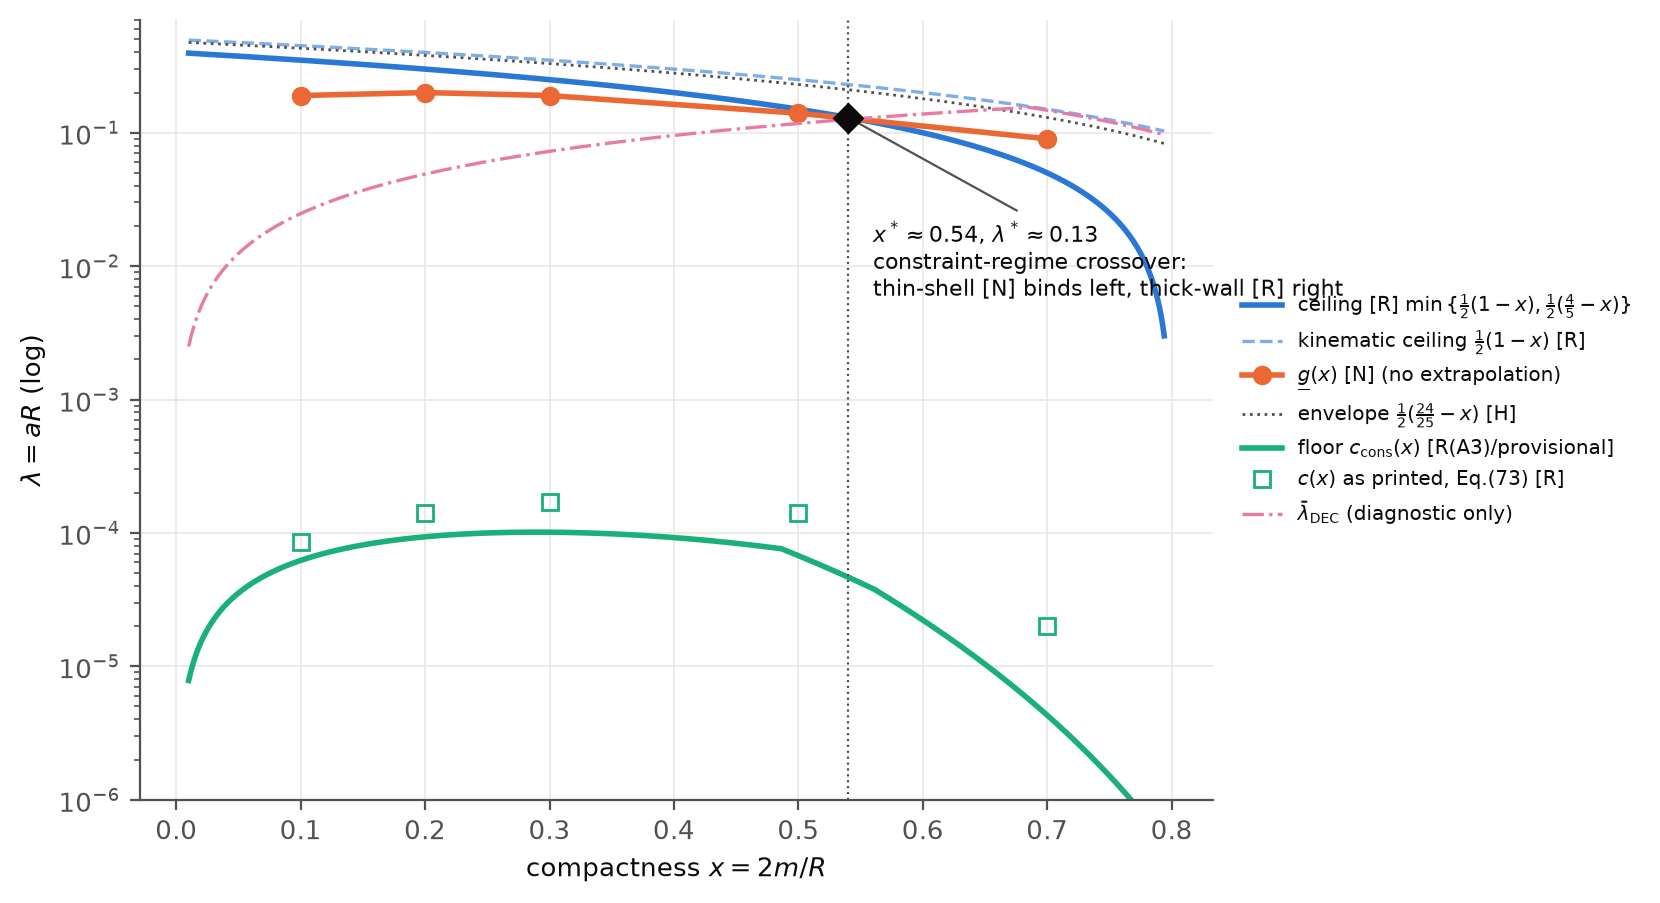
\includegraphics[width=0.95\linewidth]{figures/fig2_tiers.png}
\caption{The three-tier constraint system on $\lambda = aR$, with the
printed floor values of Eq.~(73) (open squares), our conservative floor
(solid), the effective band (circles), the ceilings, the heuristic
envelope [H], and the frozen-shape diagnostic (dash-dotted, never used as
a constraint). The diamond marks the constraint-regime crossover
$x^* \approx \NmXstar$.}
\label{fig:tiers}
\end{figure}

\begin{figure}[t]
\centering
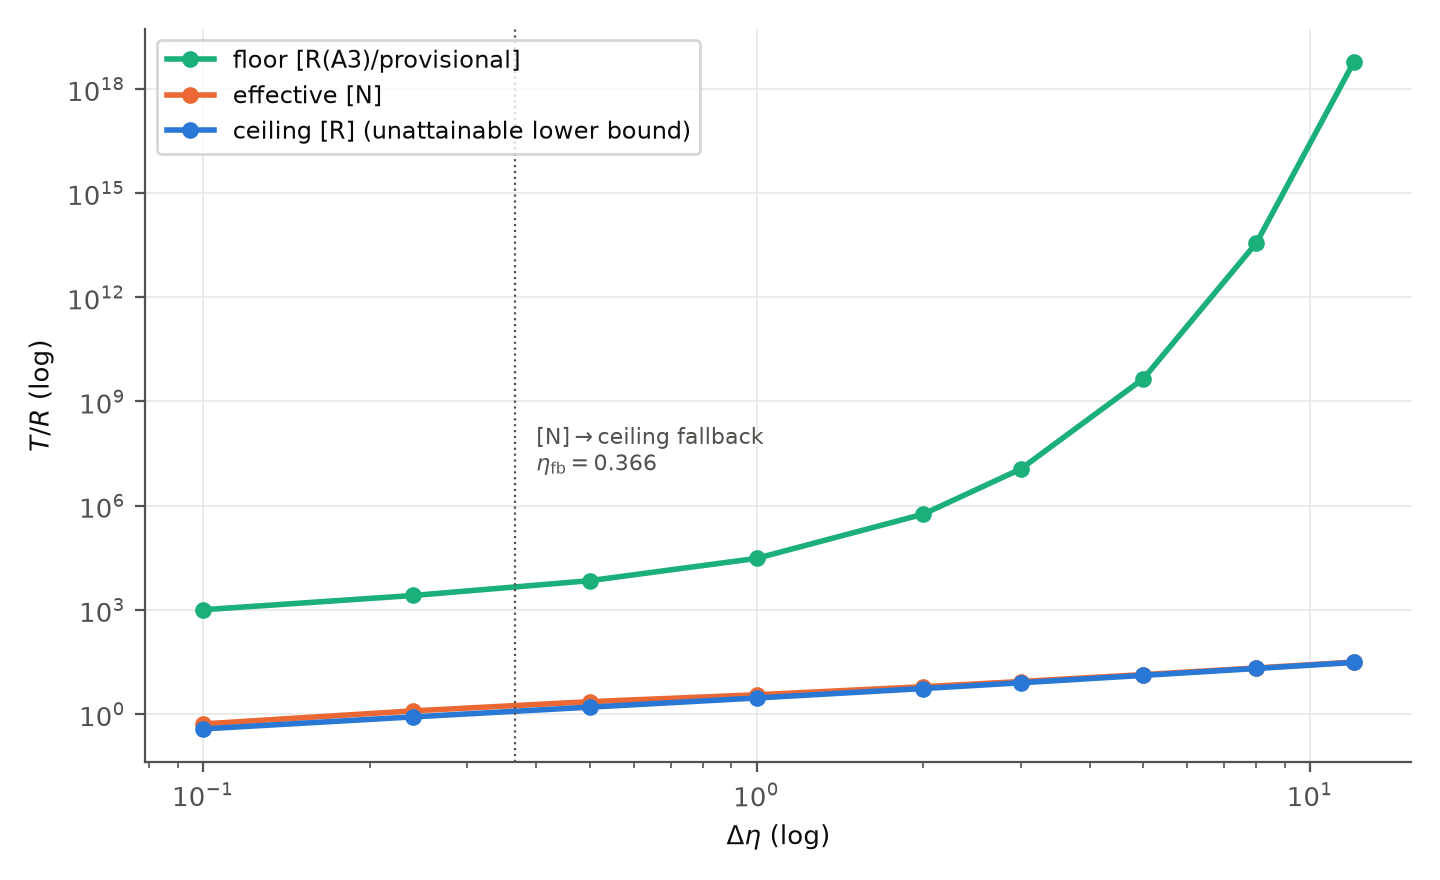
\includegraphics[width=0.8\linewidth]{figures/fig3_bracket.png}
\caption{Minimum riding time versus $\Delta\eta$ at $x_0 = 0.3$ in the
three tiers. The effective and ceiling curves converge beyond the
fallback point; the floor grows as $e^{3\Delta\eta}$.}
\label{fig:bracket}
\end{figure}

\subsection{The SI layer}

The dimensionless catalog converts to SI through a single certified
module. At $x_0 = 0.3$ and $R = 1$~km the shell mass is
$\NmMassKgKm$~kg~$= \NmMassMsunKm\,M_\odot$; the saturated riding
luminosity is $L = \tfrac32 x\lambda\,(c^5/G) = \NmLpeakW$~W
$= \NmLpeakLsun\,L_\odot$, independent of $R$; and one unit of rapidity
takes $\NmBurnMuS\,\mu$s of shell time (Table~\ref{tab:si}). A
planet-to-star-mass object burns brighter than any supernova for
microseconds at a time. The luminosity is the price the conservation law
charges for steering, paid as positive radiation.

\begin{table}[t]
\centering
\caption{SI conversions at $x_0 = 0.3$ (masses scale as $R$; the peak
luminosity $\tfrac32 x \lambda\,(c^5/G)$ is $R$-independent).}
\label{tab:si}
% AUTO-GENERATED by scripts/make_paper_numbers.py — DO NOT EDIT
\begin{tabular}{rrrrr}
\hline
$R$ [m] & $m$ [kg] & $m$ [$M_\odot$] & $L_{\rm peak}$ [W] & [$L_\odot$] \\
\hline
100 & 2.02e+28 & 0.0102 & 3.10e+51 & 8.10e+24 \\
1000 & 2.02e+29 & 0.102 & 3.10e+51 & 8.10e+24 \\
10000 & 2.02e+30 & 1.02 & 3.10e+51 & 8.10e+24 \\
\hline
\end{tabular}

\end{table}

\subsection{Observational signatures: the forward null and the
deceleration flash}

Every maneuver profile maps to observer-frame light curves through the
exact rest-frame pattern and special-relativistic aberration, Doppler
boost, and retarded-time compression, reusing the mechanics of
F\"uzfa~\cite{fuzfa2019}. Three facts organize the catalog
(Figs.~\ref{fig:fingerprint}--\ref{fig:flash}).

First, a shell accelerating at the saturated control law is exactly dark
at its forward pole: $4\pi n^2 = 3ma(1 - \cos\vartheta)$ vanishes at
$\vartheta = 0$, aberration fixes the poles, and our certification
verifies the null in exact rational arithmetic. An approaching shell is
invisible head-on for the entire boost phase.

Second, deceleration reverses the lobe: the destination observer receives
the exhaust face-on, boosted by $\delta^4 = e^{4\eta}$ and compressed in
arrival time by $dt_{\rm obs}/du = e^{-\eta}$. Along a saturated
deceleration leg the received flux follows the closed-form decay law
$F \propto e^{7\eta - 3\Delta\eta_{\rm tot}}$, obtained by combining the
boost with the Tsiolkovsky mass history; for the M31 arrival
($\Delta\eta_{\rm tot} = 24$) this is $e^{7\eta - \NmFlashExp}$, the peak
$F D^2$ is $\NmFlashPeak$ in geometric units (the catalog value agrees
with the closed form to better than $10^{-12}$), and the decay scale is
$e^{-\eta}/(7\lambda) \approx \NmFlashDecay\,R$, about $\NmFlashPs$~ps for
$R = 1$~km. Low-rapidity arrivals stretch to microseconds. The
arrival-type mission is therefore a matched pair: a departure-side burst
at $t \approx 0$ and a destination-side flash one light-crossing of the
route later.

Third, the energy closure that stitches the two layers is exact: the
integrated light curve of every profile equals $m_0 - m_f$ to $10^{-10}$
(certification C15), so the timetable and the light curve are two readings
of the same integral.

\begin{figure}[t]
\centering
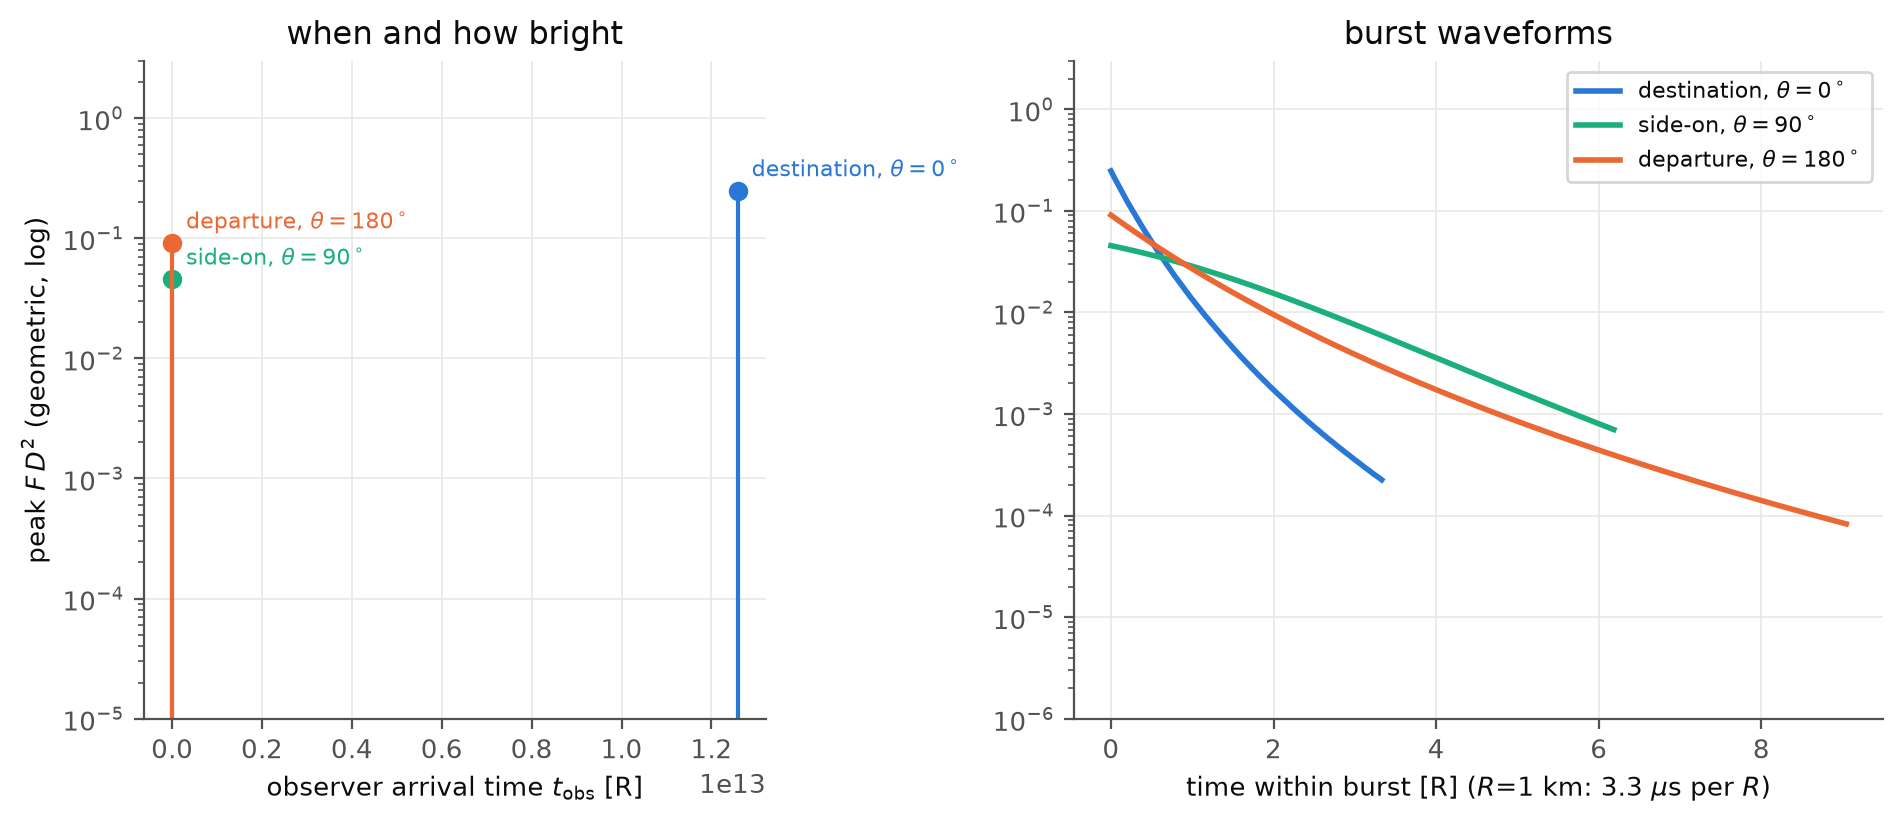
\includegraphics[width=\linewidth]{figures/fig4_fingerprint.png}
\caption{Arrival-mission fingerprint (Proxima, $\eta = 1$). Left: arrival
schedule of the transients seen by the three canonical observers. Right:
burst waveforms; the destination flash is the brightest and shortest.}
\label{fig:fingerprint}
\end{figure}

\begin{figure}[t]
\centering
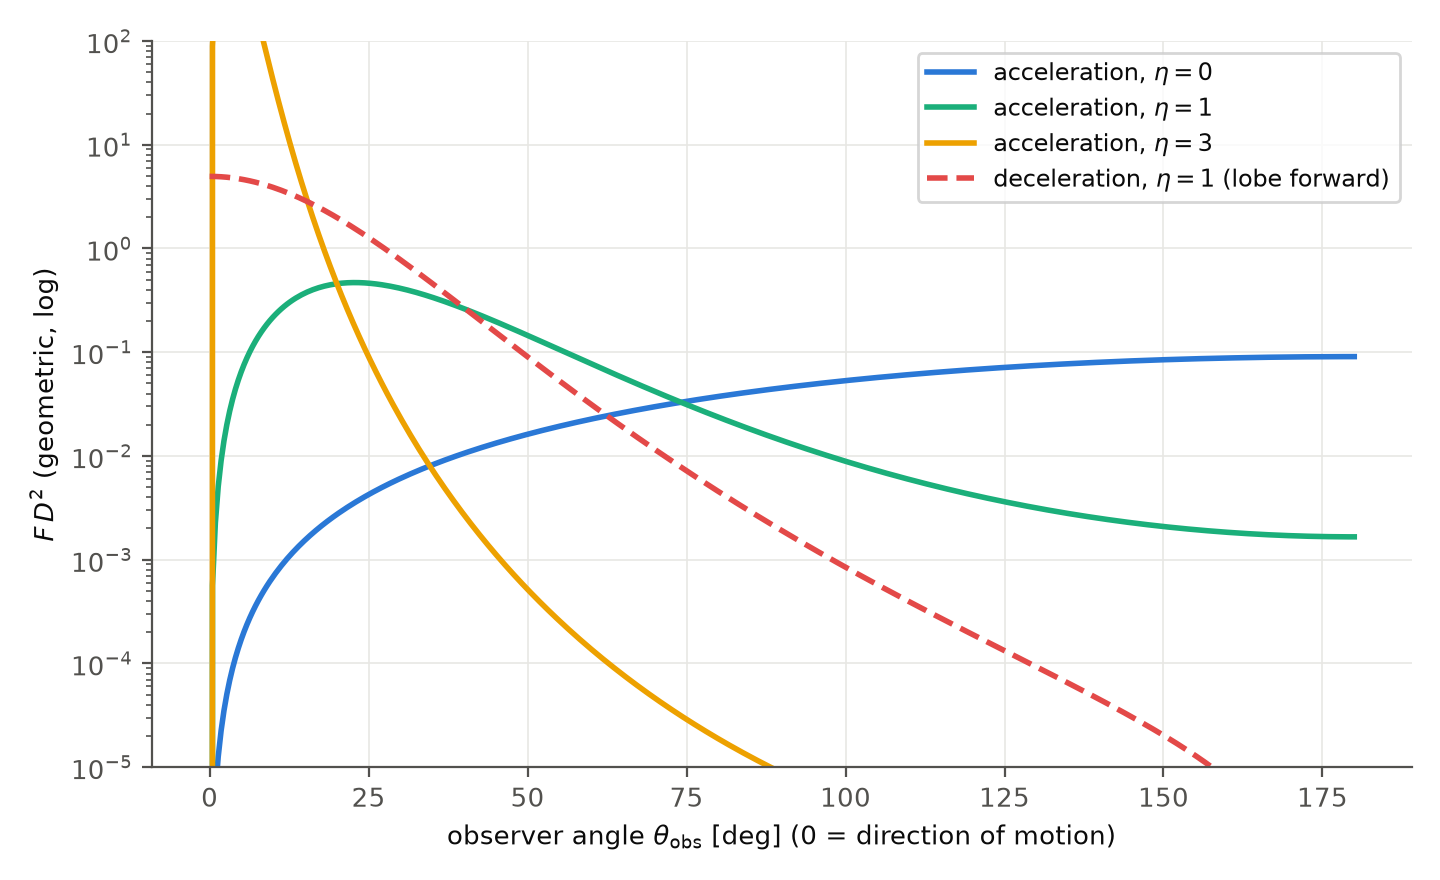
\includegraphics[width=0.8\linewidth]{figures/fig5_pattern.png}
\caption{Observer-frame angular pattern of a saturated burn at several
rapidities, and the reversed lobe of a deceleration burn. The forward null
of the acceleration pattern is exact.}
\label{fig:pattern}
\end{figure}

\begin{figure}[t]
\centering
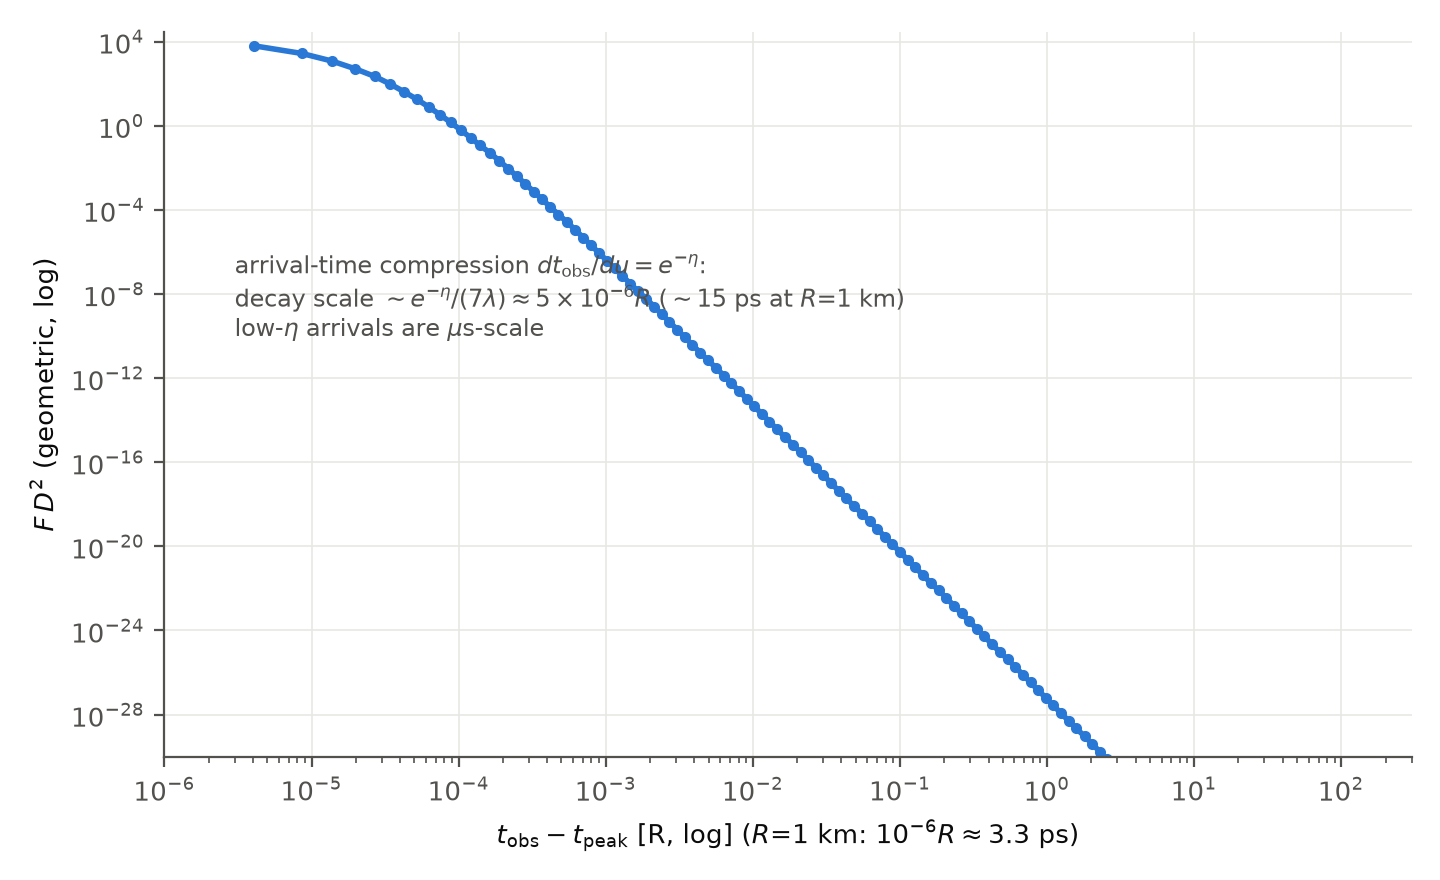
\includegraphics[width=0.8\linewidth]{figures/fig6_flash.png}
\caption{The M31 deceleration flash seen from the destination
(logarithmic time from peak). Arrival-time compression turns a
$63R$-long burn into a picosecond-scale transient.}
\label{fig:flash}
\end{figure}

\subsection{The gravitational-wave silence discriminator}

The minimum-radiation maneuver is the Damour dipole, and on that maneuver
the exterior radiates no gravitational waves: the Bondi news vanishes
identically because the spin-raising operator annihilates the $\ell \leq
1$ emission, a property established for photon rockets by
Damour~\cite{damour} and holding exactly for the news-silent class of
Ref.~\cite{le-steering}. Departures from the pure dipole radiate: the news
energy is a positive quadratic form in the $\ell \geq 2$ leakage
amplitudes, so gravitational-wave output grows quadratically while the
fuel saving from sharper collimation grows only linearly. The model
therefore makes a falsifiable joint prediction, a photometric transient
with no gravitational-wave counterpart at the same position and time, and
the same pair of channels acts as a purity meter for the maneuver itself.
The contrast with warp-drive collapse is sharp: containment failure of an
Alcubierre-class bubble emits a gravitational-wave burst as its primary
signal~\cite{clough}, the opposite corner of the discriminant plane.
Proposals to search for emissions from positive-energy warp
bubbles~\cite{lentzfelton} can draw the required waveforms and angular
patterns directly from the present catalog.

\section{Discussion}\label{sec:discussion}

\subsection{Limitations}

The catalog's validity boundaries are carried by its labels. The
accelerated thick-wall energy-condition theorem is open in the source
theory (its author states it as future work), so thick-wall realizability
is imposed as the static window on the rear-pole effective compactness.
The effective band $\underline{g}(x)$ is defined only on $x \in [0.1,
0.7]$ and is never extrapolated; riding profiles fall back to the rigorous
ceiling outside it, with fallback points recorded. Signatures are
bolometric with parameterized scenarios only (a blackbody reading of the
$R = 1$~km shell would peak in hard gamma rays, but that is a labeled
assumption, not a claim about the exhaust microphysics). The floor tier
remains provisional pending the reconciliation described in
Sec.~\ref{sec:methods}. Interpretive assumptions introduced by this work
(the dimensionless closure of the worked burn, the mission burn
convention, the floor-chain reading, and the thin-shell clamp rationale)
are enumerated in the assumptions ledger of the data release.

\subsection{Position in the time--luminosity plane}

The predicted transients occupy a corner of the time--luminosity plane
that known astrophysical classes do not: microsecond-to-picosecond
durations at equivalent isotropic luminosities far above supernova peaks,
in single events or matched pairs, with an exact forward null before
arrival and gravitational silence throughout. We make no statement about
detectability with any instrument; the physical geometry (beamed within
$\sim e^{-\eta}$, non-repeating, paired across a light-crossing of the
route) suffices to distinguish the class from repeating or
gravitationally loud phenomena at the level of scaling laws.

\subsection{Reproducibility of the floor values}

We restate the one open verification item as an invitation. The printed
floor evaluations of Eq.~(73) require three suprema whose closed forms
appear in neither the paper nor the public code at the pinned commit; our
conservative reconstruction bounds them from above under a documented
reading and lands strictly below the printed values. Publication of the
computation behind Eq.~(73) would close the gap and likely sharpen the
floor tier of this catalog.

\section{Data availability}\label{sec:data}

The full pipeline (certified library, certification suite C1--C19,
catalogs, signature files, figure and table generators, the numbers
manifest, and the assumptions ledger) is released at [GitHub URL, Zenodo
DOI to be minted at release], pinned at [commit hash injected at release]
of the project repository. The verification suite runs in under one minute
and reproduces every number in this paper.

\section*{Acknowledgments}

This work uses warpax~\cite{warpax-code} and the world\_tube reproduction
code~\cite{worldtube}, both MIT-licensed, by An T. Le. All computations,
implementations, and drafting were performed by Claude (Fable 5,
Anthropic) under the human-gated protocol described in
Sec.~\ref{sec:methods}; the human author directed the project, arbitrated
all decision gates, and bears responsibility for the content.

\begin{thebibliography}{99}
\bibitem{le-steering} A. T. Le, ``Steering a warp drive without exotic
matter,'' arXiv:2606.22531 (2026).
\bibitem{le-boundary} A. T. Le, ``On the boundary cost of source-consistent
warp shells,'' arXiv:2605.25417 (2026).
\bibitem{le-warpax} A. T. Le, ``Observer-robust energy condition
verification for warp drive spacetimes,'' arXiv:2602.18023 (2026).
\bibitem{alcubierre} M. Alcubierre, Class. Quantum Grav. \textbf{11}, L73
(1994).
\bibitem{ssv} J. Santiago, S. Schuster, and M. Visser, Phys. Rev. D
\textbf{105}, 064038 (2022).
\bibitem{pfenning} M. J. Pfenning and L. H. Ford, Class. Quantum Grav.
\textbf{14}, 1743 (1997).
\bibitem{lobo} F. S. N. Lobo and M. Visser, Class. Quantum Grav.
\textbf{21}, 5871 (2004).
\bibitem{lentz} E. W. Lentz, Class. Quantum Grav. \textbf{38}, 075015
(2021).
\bibitem{celmaster} B. Celmaster and S. Rubin, arXiv:2511.18251 (2025).
\bibitem{bobrick} A. Bobrick and G. Martire, Class. Quantum Grav.
\textbf{38}, 105009 (2021).
\bibitem{fuchs} J. Fuchs, C. Helmerich, A. Bobrick, L. Sellers,
B. Melcher, and G. Martire, Class. Quantum Grav. \textbf{41}, 095013
(2024).
\bibitem{helmerich} C. Helmerich, J. Fuchs, A. Bobrick, L. Sellers,
B. Melcher, and G. Martire, Class. Quantum Grav. \textbf{41}, 095009
(2024).
\bibitem{fuzfa2019} A. F\"uzfa, Phys. Rev. D \textbf{99}, 104081 (2019).
\bibitem{fuzfa2020} A. F\"uzfa, W. Dhelonga-Biarufu, and O. Welcomme,
Phys. Rev. Research \textbf{2}, 043186 (2020).
\bibitem{kinnersley} W. Kinnersley, Phys. Rev. \textbf{186}, 1335 (1969).
\bibitem{damour} T. Damour, Class. Quantum Grav. \textbf{12}, 725 (1995),
arXiv:gr-qc/9412063.
\bibitem{bonnor} W. B. Bonnor, Class. Quantum Grav. \textbf{11}, 2007
(1994).
\bibitem{vdgk} U. von der G\"onna and D. Kramer, Class. Quantum Grav.
\textbf{15}, 215 (1998).
\bibitem{israel} W. Israel, Nuovo Cimento B \textbf{44}, 1 (1966).
\bibitem{clough} K. Clough, T. Dietrich, and S. Khan, Open J. Astrophys.
\textbf{7} (2024), arXiv:2406.02466.
\bibitem{lentzfelton} E. W. Lentz and R. C. Felton, arXiv:2405.19381
(2024).
\bibitem{worldtube} A. T. Le, world\_tube reproduction code,
\url{https://github.com/anindex/world_tube} (MIT license).
\bibitem{warpax-code} A. T. Le, warpax v1.3.0,
\url{https://github.com/anindex/warpax} (MIT license).
\end{thebibliography}

\end{document}
